\subsection{Reliability Relevance}

\textbf{\emph{Observation}}~~ 
When an uncertain edge is altered (partial added or deleted), it will result in the change of reliability. 
The same amount of alteration performed over different edges may incur significantly different structure change. 
Referring to the example in Figure~\ref{fig:edgeRRGraph}, two vertices $\tt{a}$ and $\tt{e}$ will be assigned the same {\em uniqueness score} due to the exact probabilities associated with their edges. 
As a result, the {\em anonymity-oriented} strategy would select and perturb either of the two edges $(\tt{a},\tt{c})$ and $(\tt{c},\tt{e})$ with the same probability. 
However, the modifications to $(\tt{c},\tt{e})$---which is the only link between two~\emph{reliable} clusters---clearly incurs much larger structure distortion than that on $(\tt{a},\tt{c})$. 
Therefore, edge perturbation needs to consider the structural impact of \emph{uncertain} graph edge alteration.



To this end, we propose a theoretically sound estimation for the {\em ``reliability deviation''} caused by individual uncertain edge modifications in a fine-grained way. 
Following this path, we introduce a new measure, called {\em Edge Reliability Relevance $(\mathcal{E}RR)$}, at the edge level, and an aggregated measure, called {\em Vertex Reliability Relevance $(\mathcal{V}RR)$}, at the vertex level as will be formally defined next. These measures will enable ranking the edges to be targeted for obfuscation in a meaningful utility-based perspective. Besides, we provide an algorithm for computing them efficiently. 


\begin{definition}
    \textbf{Two-terminal Reliability Relevance}
    Given an uncertain graph $\mathcal{G}$, and two nodes $u$ and $v$, 
    the  reliability $R_{u,v}(\mathcal{G})$ as defined in Def.~\ref{d:reliability} is considered as a multivariate function involving all the edge probabilities in $\mathcal{G}$.   
    Thus, given an uncertain edge $e \in \mathcal{G}$, the partial derivative of $R_{u,v}(\mathcal{G})$ w.r.t $e$'s probability 
    variable $p(e)$, denoted as $\mathcal{E}RR^{e}_{u,v}(\mathcal{G})$, represents the sensitivity of the 
    two-terminal reliability $R_{u,v}$ w.r.t $p(e)$ while all others are held constant. 
     It is defined as:  
\begin{equation*}
	\vspace{-0.5em}
    \mathcal{E}RR^{e}_{u,v}(\mathcal{G}) = \frac{\partial R_{u,v}(\mathcal{G})}{\partial \mathit{p}(e)}
    \vspace{-0.5em}
\end{equation*}
\end{definition}


\begin{figure}
  \vspace{-1em}
    %\captionsetup{justification=centering,margin=0cm}
  \subfigure[An uncertain graph]{\label{fig:edgeRRGraph}  %(22)
    \begin{minipage}[l]{0.4\columnwidth}
      \centering
      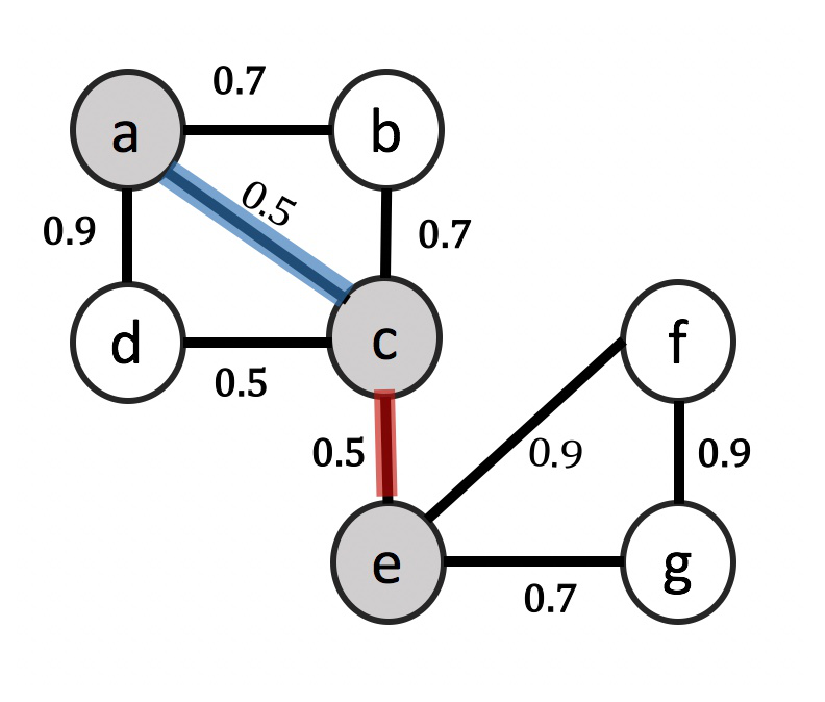
\includegraphics[height=3cm]{ill/edgeSelection.eps}
    \end{minipage}
  }
  \subfigure[The reliability $R_{a,e}$ v.s $p(e)$]{\label{fig:edgeRR}  %(22)
    \begin{minipage}[l]{0.5\columnwidth}
      \centering
      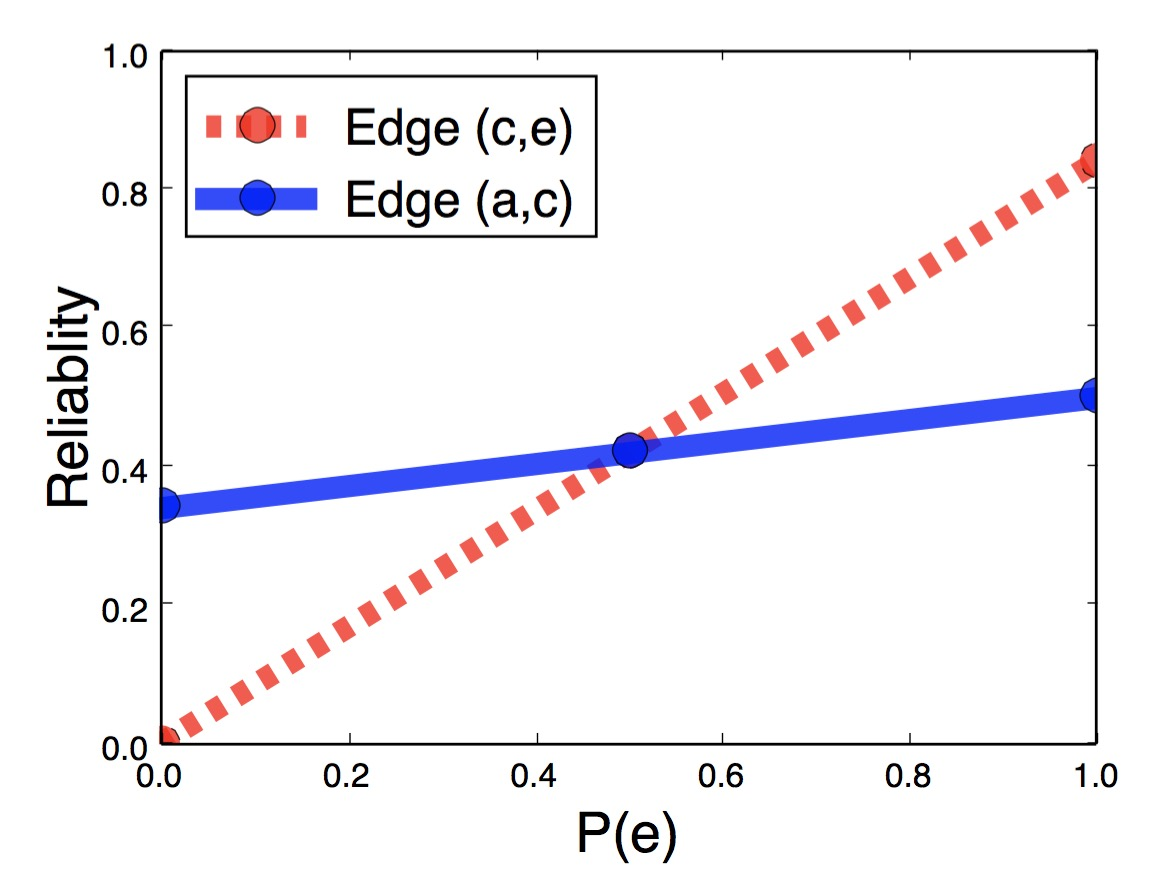
\includegraphics[height=3cm]{ill/rrIll.eps}
    \end{minipage}
  }
    \vspace{-1em}
    \caption{(a) Different edges have different effect on the overall graph reliability. (b) Formal {\em Reliability Relevance } measure. A bigger edge's slope indicates  
     big distortion in reliability under small changes to the edge's probability.}
    \vspace{-0.5em}
\end{figure}


\begin{lemma}
    \textbf{Factorization Lemma}
       Given an uncertain graph $\mathcal{G}$, the reliability of the node pair $(u,v)$, i.e., $R_{u,v}(\mathcal{G})$, can be factorized via a specific uncertain edge $e$ as follows:
    \begin{equation*}
        R_{u,v}(\mathcal{G}) = p(e) R_{u,v} (\mathcal{G}_{e}) + (1-p(e)) R_{u,v} (\mathcal{G}_{\bar{e}} ) 
        \label{eq:fac}
    \end{equation*}
    where uncertain graphs $\mathcal{G}_{e}$ and  $\mathcal{G}_{\bar{e}}$ are identical to the original graph $\mathcal{G}$ with the 
    exception that $e$ is certainly present in the former and certainly not present in the later. 
\end{lemma}


According to the factorization lemma, the partial derivative $\mathcal{E}RR^{e}_{u,v}$ can be rewritten as: 
\begin{equation*}
    \mathcal{E}RR^{e}_{u,v}(\mathcal{G}) = R_{u,v}(\mathcal{G}_{e})-R_{u,v}(\mathcal{G}_{\bar{e}})
\end{equation*}

On one hand, this factorization indicates that for a given edge $e$,  the incurred reliability discrepancy is {\bf linear} to the amount of edge probability difference. 
On the other hand, it indicates that edges with different topological locations have different reliability sensitivity. 
The other crucial point to highlight is that $R_{u,v}(\mathcal{G}_{e}) - R_{u,v} (\mathcal{G}_{\bar{e}}) \ge 0$ is always true since 
all connected pairs in $\mathcal{G}_{e}$ are guaranteed to be a superset or at least equal to that in $\mathcal{G}_{\bar{e}}$.

Considering a single uncertain edge $e$, the derivatives $\mathcal{E}RR^e_{u,v}(\mathcal{G})$ over all 
vertex pairs in $\mathcal{G}$ can be arranged in a $|V|\times |V|$ matrix, and as highlighted above, 
all entires of this matrix equal to or greater than zero.  
By aggregating these derivatives, we can estimate the overall {\em reliability relevance} of edge $e$, denoted as
$\mathcal{E}RR^{e}(\mathcal{G})$, as the sum of all the $\mathcal{E}RR^{e}_{u,v}$ values. That is:
%In this work, we define $RR(e)$ to be reliability relevance of an edge $e$ which can be quantified by the sum of all the $RR_{u,v}(e)$, as  
\begin{align*}
    \mathcal{E}RR^e(\mathcal{G}) &= \sum_{u,v} |\mathcal{E}RR^e_{u,v}(\mathcal{G})| \\
          &= \sum_{u,v} |R_{u,v}(\mathcal{G}_{e}) -R_{u,v}(\mathcal{G}_{\bar{e}})| \\  
         &= \sum_{u,v} R_{u,v} (\mathcal{G}_{e}) - \sum_{u,v} R_{u,v}(\mathcal{G}_{\bar{e}}) 
\end{align*}

Note that $\mathcal{E}RR^e$ equals to the difference of the expected number of 
connected pairs between the two uncertain graphs $\mathcal{G}_{e}$ and $\mathcal{G}_{\bar{e}}$
 by explicit incorporation of edge uncertainty.  
 In the context of edge relevance, reliability relevance can be seen as generalization of cut-edges, 
 which quantifies the impact of partial edge deletion or addition on the connectivity in the uncertain graph. 
The higher reliability relevance score of an edge, the bigger impact of edge perturbation over the overall graph.  

On the basis of these edge-level reliablity relevance, we can now compute a vertex-level reliability relevance of a given vertex (Say $u$) as a weighted sum of reliability relevance of $u$'s edges $\mathtt{E}^{u}$.  
% Fix $u \in \mathcal{G}$ and let $\mathtt{E}^{u}$ be the pairs of vertices that include $v$, we have 
\begin{equation*}
    \vspace{-0.5em}
    \mathcal{V}RR^{u}(\mathcal{G})=\sum_{e \in \mathtt{E}^{u}} p(e)  \mathcal{E}RR^{e}(\mathcal{G})
    \vspace{0.5em}
\end{equation*}

The $\mathcal{V}RR^{u}(\mathcal{G})$  is a measure of the expected impact of vertex modification on the graph reliability. Namely, the higher the vertex's reliability relevance, the larger reliability distortion introduced by modification associated with its edges.

\textbf{Reliability Relevance Evaluation}
Given this theoretical foundation, the challenge is how to evaluate the reliability relevance of edges in  a given uncertain graph efficiently ($\mathcal{E}RR-$eval). 
For each edge $e$, we need to measure the reliability difference over $\mathcal{G}_{e}$ and $\mathcal{G}_{\bar{e}}$. 
This evaluation involves the two-terminal reliability detection problem, which is known to be NP-complete~\cite{MOBall}.   


A baseline algorithm for $\mathcal{E}RR-$eval is to use the
Monte Carlo sampling. More precisely, we sample $N$ possible
worlds of the input uncertain graph, where $N$ is large enough (around $1,000$) to guarantee high approximation accuracy. 
Over each sampled possible world (Say $G$), we carry out a connected-component computation algorithm to count 
the number of connected pairs $cc(G)$. Then, the count on the original uncertain graph $cc(\mathcal{G})$ can be estimated by taking the average over the sampled deterministic graphs. 

\begin{theorem}
	The complexity of the baseline $\mathcal{E}RR-$eval algorithm is $\mathcal{O} (|E| \cdot  N \alpha(|V|) |E| )$ where $\alpha$ is the inverse Ackermann function.  
\end{theorem}

{\bf Proof sketch} The time complexity of the connected component detection algorithm based on the union-find method is $\mathcal{O}(\alpha(|V|) |E|)$~\cite{Wredman:1989:CPC:73007.73040}. Consequently, computing the $\mathcal{E}RR$ for an edge over the $N$ possible worlds takes time $\mathcal{O}(N \alpha(|V|) |E|)$, and the total time complexity for all the edges is $\mathcal{O} (|E| \cdot  N \alpha(|V|) |E|)$. 


\begin{figure}
	\centering
    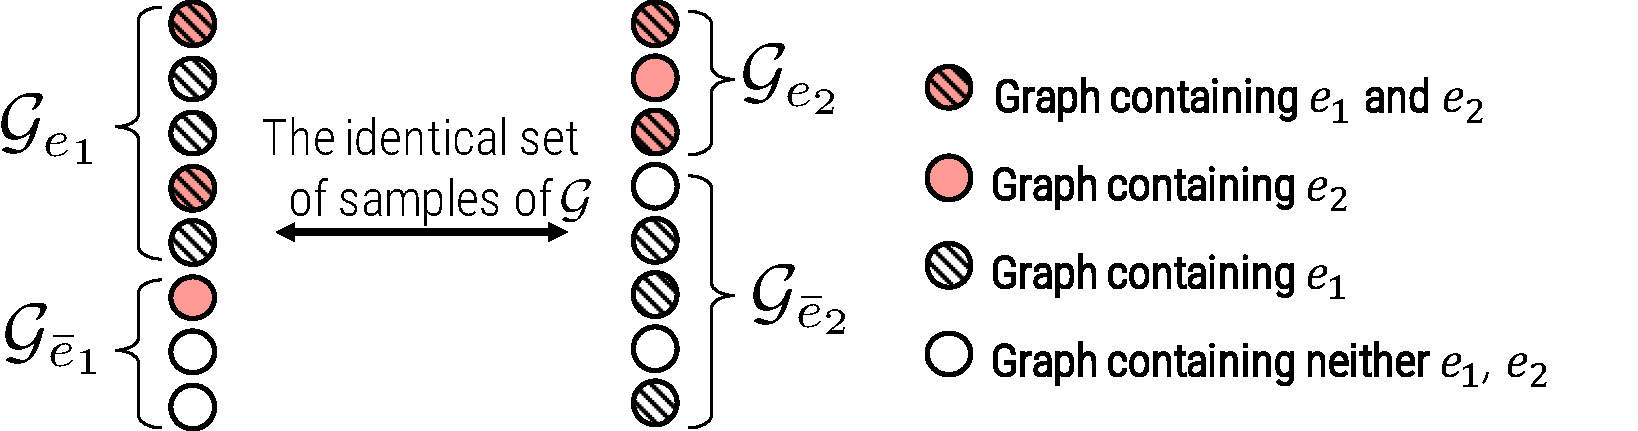
\includegraphics[width=1\linewidth]{ill/rrEval.pdf}
    \vspace{-1em}
    \caption{\small Reused sampling estimator for $\mathcal{E}RR$ }
    \label{fig:rrEval}
%     \vspace{-1em}
\end{figure}
Obviously, the baseline algorithm is inefficient when the input uncertain graph is very large (it is quadratic in the number of edges). Here, we present a efficient algorithm for $\mathcal{E}RR$ evaluation in Algorithm~\ref{alg:RReval}. Its basic idea is to re-use the connected components detection result of samples as illustrated in~\ref{fig:rrEval}. For each edge $e$, we group the sampled possible worlds according to the edge existence (Line 4-6), then get the sampled average of $cc$ for each group as accurate approximation of $cc(\mathcal{G}_{e})$ and $cc(\mathcal{G}_{\bar{e}})$. By this way, we bring the the evaluation of edge reliability relevance to the realm.  

\begin{theorem}
	The time complexity of Algorithm\ref{alg:RReval} $\mathcal{E}RR-$val is $\mathcal{O}(N \alpha(|V|) |E|)$ where $N$ is the number of samples.
\end{theorem}



\begin{algorithm}[!tb]
{\scriptsize
    \begin{algorithmic}[1]
       \item[] {\textbf{Input:} ~$\mathcal{G}=(V,E,\mathit{p})$, $N$ is the number of sampled graphs;~}
       \item[] {\textbf{Output:} ~$\mathcal{E}RR$ Reliability relevance of edges in $\mathcal{G}$}
    \STATE {$CC_{e} \leftarrow  \mathbf{0} $, $CC_{\bar{e}} \leftarrow \mathbf{0}$}
    \FOR{i=1 \TO N }
    \STATE {$G \leftarrow $  A deterministic sampled instance}
    \STATE {$Ind(G)$ is edge existence of sampled graph $\mathcal{G}$}
    \STATE {$cc(G) \leftarrow $ the number of connected pairs of $G$}
    \STATE {$CC_{e}+=Ind(G) \cdot cc(G)$,$CC_{\bar{e}}+=(\mathbf{1}-Ind(G)) \cdot cc(G)$ }
    \ENDFOR
    \STATE{$\mathcal{E}RR= CC_{e}/\mathit{p} - CC_{\bar{e}}/{\mathbf{1}-\mathit{p}}$}
         \caption{Edge Reliability Relevance Evaluation}
        \label{alg:RReval}
    \end{algorithmic}
    }
\end{algorithm}
